\section{Final confirmation: relation benefit, information transfer, and convergence}
\subsection{Budget-controlled correspondence benefit}
Table~\ref{tab:final} reports all original arms and the separate convergence and transfer diagnostics.
GELU's correct-minus-incorrect collision advantage is +11.88 pp [+8.05, +15.62].
The activation-by-correctness interaction is +12.89 pp [+8.67, +17.03].
Its direction is positive in all five new sources. Budget-linear correct-minus-incorrect performance is -1.02 pp [-3.75, +1.80].
All four budget arms have 100\% first-generator accuracy on the collision set.
Thus matching the winning first-step answer is insufficient to explain the compound-performance differences.

\begin{table}[ht]\centering\small
\begin{tabular}{lrrrr}\toprule
First-state predictor & AB (\%) & Both (\%) & A (\%) & State NMSE\\\midrule
Budget linear, correct & 8.44 & 0.47 & 100.00 & 0.04647 \\
Budget linear, incorrect & 9.45 & 0.31 & 100.00 & 0.06859 \\
Budget GELU, correct & 20.31 & 5.00 & 100.00 & 0.01973 \\
Budget GELU, incorrect & 8.44 & 1.09 & 100.00 & 0.06874 \\
Converged affine, correct & 19.92 & 3.75 & 99.84 & 0.02963 \\
Converged affine, incorrect & 8.36 & 0.31 & 99.77 & 0.08200 \\
Linear + correct GELU null & 17.19 & 2.66 & 100.00 & 0.03744 \\
Linear + incorrect GELU null & 8.75 & 0.47 & 100.00 & 0.06818 \\
GELU + linear null & 13.20 & 1.56 & 100.00 & 0.02876 \\
\bottomrule\end{tabular}
\caption{Final collision test averaged over five independent source initializations. Both requires both members of a collision pair to be correct. Converged affine fitting receives additional optimization budget; hybrid states are predicted-component interventions. State NMSE uses the fixed training variance, not displacement energy.}\label{tab:final}
\end{table}

The correct GELU compound accuracy is 20.31\%, and pairwise double correctness is 5.00\%.
These are local improvements; stable inference above the three-gold-answer-only 50\% ceiling is not established.
True-intermediate composition averages 99.06\%, showing that a reliable second map exists when supplied the actual intermediate.
This oracle result is a diagnostic, not a predictor.

\subsection{A predicted component transmits functional benefit}
For the fixed full first-step linear readout, let $P$ project onto its row span and $Q=I-P$.
We construct
\[
 \hat h_{L\leftarrow G}=\hat h_LP+\hat h_GQ.
\]
The donor and recipient are their own predicted first states in the same frozen source coordinates. No true intermediate enters the swap.
Because $QW^\top=0$, all recipient first-step logits are preserved.
The maximum measured logit change across the interventions is $2.23\times10^{-13}$.

A correct GELU donor raises the correct linear recipient from 8.44\% to 17.19\%, an increment of +8.75 pp [+5.31, +12.42].
The same swap with an incorrect GELU donor reaches 8.75\%.
The correct-minus-incorrect donor contrast is +8.44 pp [+4.92, +11.95], positive in every source.
Reverse replacement of the correct GELU null component by the linear one lowers GELU performance to 13.20\%.
This supports a correspondence-sensitive functional pathway through predicted information invisible to the fixed first readout.
It does not identify that subspace with all answer-independent information, or guarantee that hybrid states lie on the encoder manifold.

\subsection{Adequate affine fitting changes the interpretation}
Identity residuals express the unrestricted affine family. We therefore optimize that family directly under Equation~\ref{eq:loss}, retaining the same correct teacher logits, geometric targets, geometry coefficient, and zero regularization.
Float64 SVD whitening conditions the training design; readout-null coefficients take their least-squares optimum, while readout-row coefficients are optimized by L-BFGS.
Both OLS and budget-linear row initializations were fixed before final training.
No compound labels, states, or checkpoint selection enter fitting.
Appendix~\ref{app:convergence} details the objective and numerically evaluated gradient-based convergence bounds.

Converged correct affine prediction reaches 19.92\%, and its correct-minus-incorrect gain is +11.56 pp [+6.56, +16.80].
The remaining GELU-versus-converged-affine relation-advantage interaction is +0.31 pp [-5.86, +6.33].
Its interval crosses zero. We did not confirm an additional functional expressivity advantage in this unregularized comparison; neither does this establish equivalence. The later validation-selected ridge sensitivity analysis restricts this conclusion further (Section on reviewer revisions).
Correct affine improvement over the original budget-linear arm is +11.48 pp [+6.56, +16.56].
This is a same-family optimization diagnostic with changed parameterization, precision and budget, rather than another budget-matched causal comparison.
GELU retains a smaller first-state NMSE (0.01973 versus 0.02963); total state-fitting differences alone do not determine compound accuracy.

\begin{figure}[ht]\centering
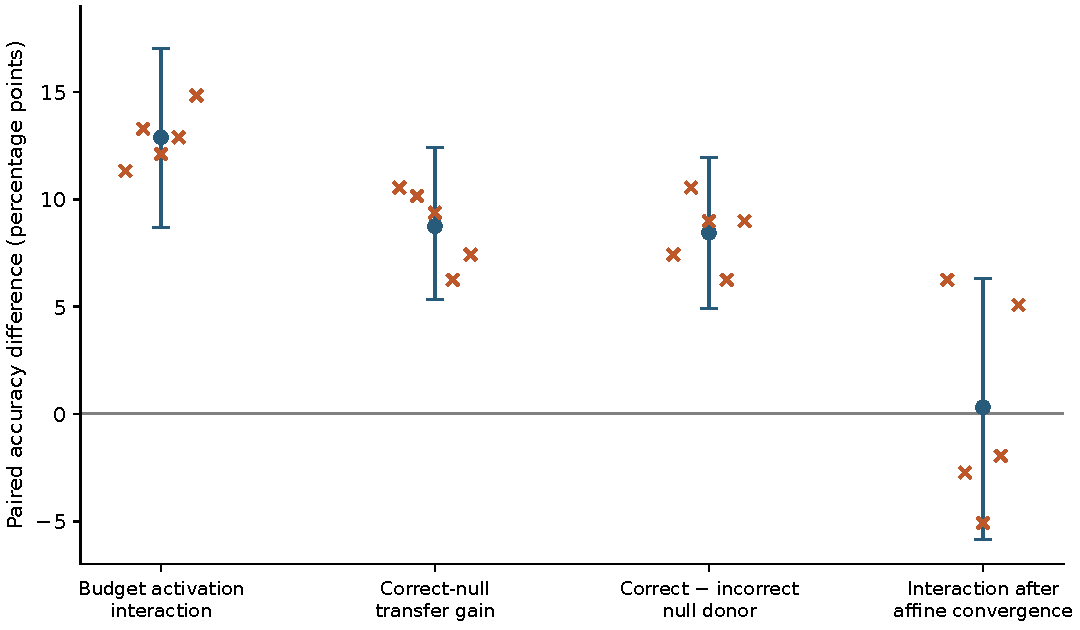
\includegraphics[width=.95\linewidth]{figures/final_contrasts.pdf}
\caption{All five source effects and descriptive crossed source/pair 95\% intervals for predeclared contrasts. Convergence narrows the original activation-by-correctness interaction.}\label{fig:contrasts}
\end{figure}

\subsection{Convergence and precision qualifications}
All twenty affine fits pass the registered convergence threshold. The largest independently recomputed training-objective gap bound is $3.87\times10^{-12}$.
The two initializations give identical compound classes; their largest first-state difference is $6.55\times10^{-5}$.
However, design condition numbers range from $8.65\times10^{7}$ to $1.29\times10^{8}$, and coefficient norms from $8.01\times10^{5}$ to $1.69\times10^{6}$.
Complete float32 replay of the affine, second-operator, and readout pipeline changes 12/1280 correct-pairing and 43/1280 incorrect-pairing collision predictions relative to float64.
Aggregate correct/incorrect accuracy is 19.92/8.36\% in float64 and 19.92/8.44\% in float32.
The aggregate correspondence benefit survives this precision check, while individual predictions are numerically sensitive.
LayerNorm's exact affine constraint makes finite-precision rank effects a remaining candidate explanation.
Convergence of the empirical objective does not guarantee numerically robust state identification or out-of-distribution stability.
